\section{Introduction}
\label{sec:intro}

% Fig. 1: panel (a) of figures/figure1.pdf (exported from figures/figure1_lavq_editable.pptx), cropped to figures/figure1_a.pdf.
\begin{figure}[t]
  \centering
  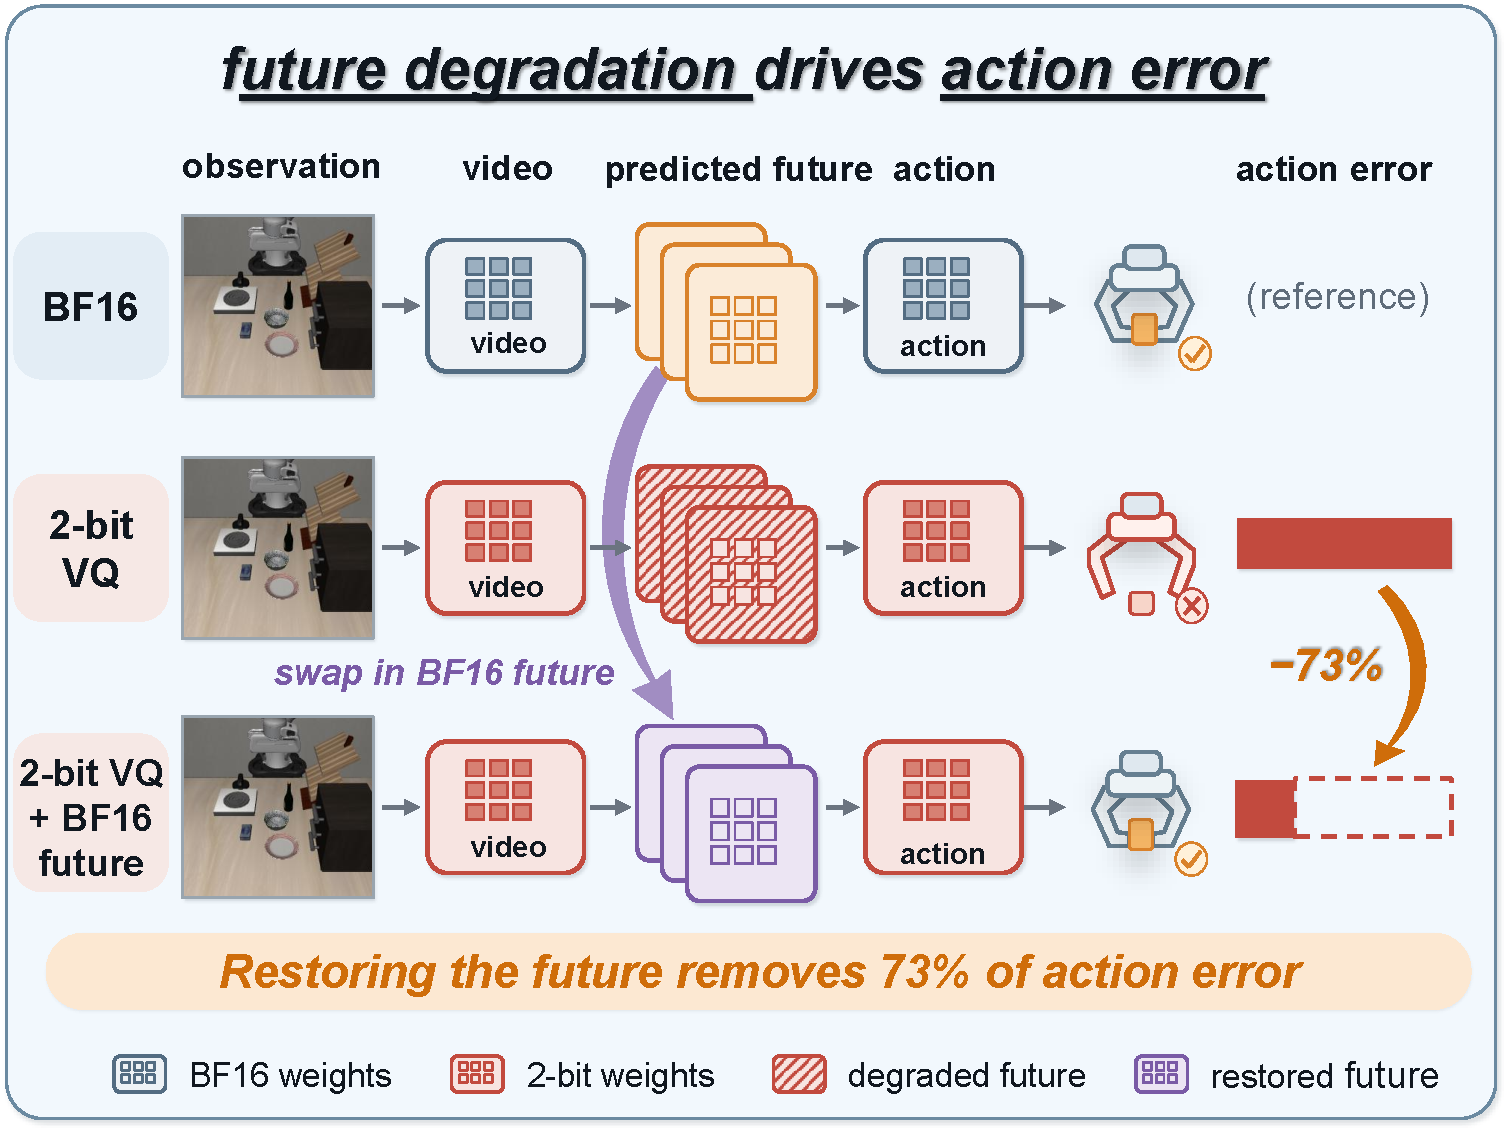
\includegraphics[width=\linewidth]{figures/figure1_a.pdf}
  \caption{Under 2-bit vector quantization, a WAM's predicted future degrades, and most of its action error follows from it: swapping in the full-precision future removes 73\% of the action error (Fast-WAM, QTIP).
  \method makes the predicted future an explicit quantization target and achieves the highest 2-bit closed-loop success on both WAMs (\cref{tab:main}).}
  \label{fig:teaser}
\end{figure}

World action models (WAMs) jointly predict how a scene will evolve and how to act~\cite{yuan2026fastwam,kim2026cosmospolicy,li2026lingbotva,ye2026dreamzero}.
Trained together with a video generator, they condition their actions on a predicted future and inherit the visual priors of large video backbones, which has made them a strong family of robot policies.
They also inherit the size of those backbones.
Fast-WAM~\cite{yuan2026fastwam} has 6B parameters, and its BF16 weights alone occupy 12\,GB, which must share the memory of an onboard computer (\eg, \XX) with the policy's activations and the rest of the robot stack.
Weight memory is therefore the first barrier to running a WAM on the robot itself, and removing it requires compressing the weights to two or three bits each.

At two to three bits per weight, the choice of quantizer is decisive.
On Fast-WAM, scalar GPTQ~\cite{frantar2023gptq} collapses at 2 bits, while vector, lattice and trellis quantizers (GPTVQ~\cite{vanbaalen2024gptvq}, QuIP\#~\cite{tseng2024quipsharp} and QTIP~\cite{tseng2024qtip}) keep the policy usable (\cref{sec:exp:main}).
These quantizers were developed for large language models.
They round each layer to minimize a reconstruction error weighted by input statistics~\cite{frantar2023gptq,egiazarian2024aqlm,vanbaalen2024gptvq,tseng2024quipsharp,tseng2024qtip}, and in this sense treat a WAM as a generic network.
Recent work on WAM quantization~\cite{zhou2026quantwams,akbari2026qwam,wang2026steerquant} targets 4-bit weights and activations and keeps the final action faithful.
None of these methods deliberately protects the predicted future on which the action depends.

We find that this omission is costly: applied to a WAM, existing VQ methods fail to preserve the fidelity of the predicted future, and the loss propagates to the action.
Three observations on Fast-WAM make this concrete (\cref{sec:motivation}).
First, most of the action error comes from a degraded future: restoring the predicted future to full precision removes 73\% of the action error of a 2-bit model and 85\% of that of a 3-bit model (\cref{fig:teaser}).
Second, future error originates in the modules that generate the future: raising them by one bit recovers 71\% of what an extra bit can buy, whereas the modules that only read the future leave it unchanged.
Third, the action reads a narrow part of the future: its sensitivity concentrates on about 42 effective directions of a 37{,}632-dimensional latent.
In closed loop, the three VQ methods lose \XX--\XX percentage points of success at 2 bits relative to BF16 on LIBERO-Plus~\cite{fei2026liberoplus}.
Preserving a WAM at ultra-low bit widths therefore requires treating the predicted future, as the policy reads it, as a quantization target in its own right.

Building on this diagnosis, we propose \method, a latent-aware vector quantization framework for WAMs (\cref{fig:method}).
We call \emph{reader} the part of a WAM that maps the predicted future to the action.
\method (i) measures future error in the metric through which the reader sees it, (ii) distributes a fixed bit budget according to each module's measured impact on future fidelity, (iii) initializes the codes with trellis-coded rounding~\cite{tseng2024qtip}, which natively supports the resulting mixed bit widths, and (iv) calibrates the shared decode tables toward action and future fidelity.
Each component answers one of the observations above.
The quantized model runs a standard trellis decoder, and the calibrated tables add no storage.

We evaluate \method on \XX WAMs in simulation and on a real AgileX PiPER arm.
On LIBERO-Plus, 2-bit \method raises the success rate of Fast-WAM from \XX\% (QTIP, the strongest 2-bit baseline) to \XX\%, within \XX points of BF16 (77.6\%), and \XX on \XX (\cref{tab:main}).
On three real-world tasks (two-object pick-and-place, pouring and cloth folding), it succeeds in \XX/\XX trials, compared with \XX/\XX for QTIP. In summary, our contributions are threefold:
\begin{itemize}
  \item We identify future-latent fidelity as a key quantization target for WAMs. Counterfactual future swaps and module-level bit upgrades show that most of the action error under ultra-low-bit quantization comes from a degraded predicted future, that this degradation originates in the modules that generate the future, and that the policy reads only a narrow part of it.
  \item We propose \method, a latent-aware vector quantization framework whose error metric, bit budget and calibration objective all follow from this finding, at the same bits per weight as the baselines and with no extra storage.
  \item We evaluate \method across \XX WAMs in simulation and on a real robot arm, where at 2 bits per weight it \XX.
\end{itemize}
